\section{A Technique for Debugging A Distributed R-Tree}
\label{sec:rdebug}

	Spatial index debugging is a big challenge in a distributed R-Tree and this section describes a new technique RDebug, which allows debugging the index building of an R-Tree.
	
	The R-tree index building follows a top-down approach, in other words, the index is always built from root to leaves. Debugging the index reliability as the index is built is a non-trivial task, and the aim of this paper is to show a technique for index debugging after it has been created. Common challenges when working with an R-Tree are: i) Reliability of the nodes replicas of the R-Tree, ii) ensure that the MBR of the parent nodes intersect the MBR of their children, iii) the existence of duplicated nodes or being referenced by more than one parent node, and iv) if the value M and m of the nodes are compliant with the R-Tree descriptions as shown in Section \ref{sec:spatial_dist}. Furthermore, it is possible to access index data to help in its optimization as dead space and overlapping area.

	Algorithm \ref{alg:rdebug} shows the RDebug technique for debugging the distributed spatial index, using the index structure itself. The algorithm has two steps:
1) The algorithm processing is similar to the search in an R-Tree; 2) The algorithm does the inverse of a search in an R-Tree appending information to the distributed index.

	The first step, called S1 [Search sub-trees] (lines 1 - 11), the Algorithm \ref{alg:rdebug} traverses every node of the R-Tree starting from the root node to the leaves. Its purpose is to spread the debugging algorithm. The first request is sent to any server, which stores a replica of the root node.

	If the node $T$ is not a leaf (lines 2 - 8), then the number of children entries is stored to control the number of expected answers to this node in the second step of the algorithm. This information is stored in a shared memory accessed by all servers with a replica of $T$. Lines 4 -7, show that for every entry $E$ in the node, a message is sent (continuing step S1) to any server that holds a replica of the child node of $E$, carrying on the first step in the children nodes. If the node is a leaf, the second step, named S2 [Aggregation] is started.

	Second step aim (lines 12 - 39) is to aggregate the information used for future debugging. This step receives the debugging information of every child node of $T$. Therefore, for a given node $T$ with $n$ children, the second step is invoked $n$ times in the node $T$.

	The index itself is used to aggregate this information, the computational resources of the cluster helps improve the debugging information aggregation time. The index reverse structure allows, besides of spanning the aggregation information processing, build the debugging aggregation information, as one node of the R-Tree is responsible to aggregate only the information of its children. 

	The information of the children nodes are stored in a shared memory, with concurrency control, by the replicas of $T$. Hence, line 13, those information are retrieved from the shared memory. Line 14 verifies the consistency of $T$ in the servers that store any replica of $T$. Line 15 verifies the consistency of $M$ and $m$ values. Lines 16 and 17 calculate the overlap and the dead space area for each node of the R-tree, respectively. Those information help the insertion algorithm designer analyze the quality of the built index. Line 18 get the MBR of the $T$. This data are inserted in $informations$ on line 18. This informations will be used as an input to a tool capable of visualizing the index of the R-Tree.
	
	If the aggregation step is being executed in the leaves (lines 20 - 24), then if  $T$ is the root node (line 22), the node information are sent to the client application. If $T$ is not the root node, in line 24, the information are sent to the parent node of $T$. If the aggregation step is in an internal node (lines 26 - 39), the algorithm aggregates the information of the children nodes. In the line 29, the algorithm receives the information sent by the child node. Line 27, verifies if the MBR of the entry that points to the child node is indeed the same MBR sent by the child node.
	
	Line 28 adds the data processed from lines 26 and 27 in $informations$. Line 29 acquires the number of children nodes that not sent debugging information yet. This value is stored in the variable $count$, which is decremented and the values is stored on shared memory to let the other replicas know.
	
	If every node has sent the answer, the variable count then will hold the value 0 and lines 30-35 are processed. If $T$ is the root node, then the information are sent to the client application, otherwise, those information are sent to the parent node of $T$. If the variable $count$ is greater than 0, then the client information are stored in the shared memory to be used until every child node send replies.	
		
\medskip
\begin{center}
\begin{minipage}{1\textwidth}
\begin{algorithm2e}[H]
\SetAlFnt{\small\sf}
 \DontPrintSemicolon
 \LinesNumbered
\SetAlgoLined
 \BlankLine
 \Entrada{$T$ reference to root node of R-Tree $tree$}
 \Saida{Debugging information about distributed R-Tree $tree$}
 \BlankLine
	
 S1 [Search subtrees]

\eIf{$T$ is not leaf}{
  store the number of child entries in each replica server of T\;
	
	\For{each entry $E$ in $T$} {
		$server \leftarrow $ choose one server, randomically,  that store one replica of $E$\;
		send msg to $server$ to process the node child of $E$ on step S1\;
	}
}
{
  verifiy the consistency of $T$ in others replicas\;
	Invoke step S2 [Aggregation]\;
}

S2 [Aggregation]

$informations \Leftarrow$ the childs information stored on shared memory by replicas of $T$\;
$replica\_consistency \Leftarrow$ verifiy the consistency of $T$ in others replicas\;
$node\_consistency \Leftarrow$	verify the consistency of $M$ and $m$ values of  $T$\;
$overlap \Leftarrow$ overlap area of $T$\;
$dead\_area \Leftarrow$ dead area of $T$\;
$bound \Leftarrow$ MBR of $T$\;
add in $informations$: $replica\_consistency$, $node\_consistency$, $overlap$, $dead\_area$, $bound$\;

\eIf{$T$ is leaf}{
 \If{$T$ is root}{
		send response with R-Tree nodes information to app client\;
	}
	{
		send msg with $informations$ to parent of $T$\;
	}
}
{
	  $entry\_info \Leftarrow$ information sent by child node\;
    $mbr\_consistent \Leftarrow$ verify if the bound of the child node is equal to bound of entry of T that points to this child\;
    add in $informations$: $entries\_info$, and $mbr\_consistent$\;
		$count \Leftarrow$ retrieve the number of entries child which not sent a debugging response and decrement by 1 unit\;
		
    \eIf{$count$ == 0}{
        \eIf{$T$ is root}{
           send response with $informations$ to app client\;
        }
				{
				   send msg with $informations$ to parent of $T$\;
				}    
		}
		{
			store $informations$ on shared memory\;
		}
            
}
\caption{$RDebug(T)$ 
\label {alg:rdebug}}
\end{algorithm2e}
\end{minipage}
\end{center}

The algorithm \ref{alg:rdebug} was implemented in the DistGeo platform to collect the debugging information of the built distributed R-tree. Those information are used in the platform to find out indexing issues and to optimize the R-tree index for searching. With the aid of RDebug \ref{alg:rdebug} algorithm, it is possible debug the searching algorithms of an R-Tree. E.g: The Window Query algorithm shown on Section \ref{sub:spatialdata}. To tweak RDebug to Window Query, it is only needed add an window query in the first step and gather the aggregation information of the accessed nodes. Whereas, the algorithms that access diverse R-Trees, such as Spatial Join, need a deep change, as the algorithms can go through different paths.

Figure \ref{fig:rdebug-vis} shows a graphical tool (RDebug Visualizer) created to visualize the structure of the distributed R-Tree index, using as the input the information generated by the distributed debugging algorithm in DistGeo platform. The RDebug Visualizer allows analyze the debug information in each node of the R-Tree. The output of the RDebug algorithm notify which nodes is currently inconsistent, so the user can access the path of the node and visualize the node inconsistent information.    

\begin{figure}
	\centering
		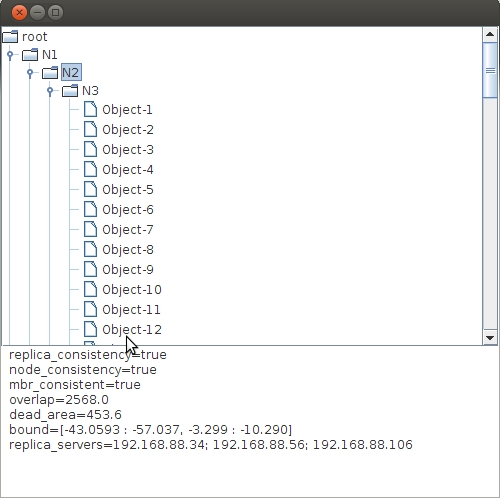
\includegraphics[width=0.5\textwidth]{rdebug-vis.jpg}
	\caption{RDebug Visualizer}
	\label{fig:rdebug-vis}
\end{figure}


